\newpage
\section{Introducc\'ion}

Utilizando verilog, se realiza un proyecto para la entrega del trabajo final de la materia arquitectura de computadoras 2012. El proyecto consiste en la construcción de un pipeline de 5 etapas capaz de decodificar un código previamente cargado y que este sea capaz de procesarlo, llegando hasta la ejecución, por último con fines de evaluación y verficaci\'on embeber el c\'odigo desarrollado en una fpga y correr un programa desarrollado que demuestre el funcionamiento.

\subsection{IDE}
El entorno de desarrollo utilizado para el desarrollo del c\'odigo del pipeline es el \texttt{Project Navigator, release version 14.4 (lin), Aplication version:P49d}.
Para desarrolar la interfaz gr\'afica de debug se utiliz\'o el editor de interfaces \texttt{glade} y se programo la recepci\'on de datos en \texttt{python 2.7}. 

\subsection{SVN}
Se llev\'o a cabo el desarrallo del software utilizando un servidor svn para el control de cambios que facilit\'o muchisimo la tarea a la hora de volver hacia ``c\'odigo estable'' y desde alli retomar el desarrollo.

\subsection{Placa de desarrollo}
Para embeber el c\'odigo se utiliz\'o la placa de desarrollo de \texttt{Digilent, Nexys™3 Spartan-6 FPGA Board} con frecuencia de 100 MHZ, las caracter\'isticas de la placa se detallan en la figura \ref{fig:digilent}.
\begin{figure}[H]
\centering
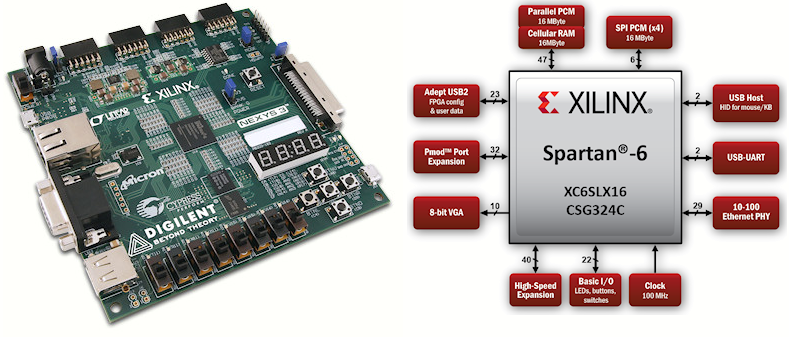
\includegraphics[scale=0.35]{img/digilent}
\caption{Placa de desarrollo}
\label{fig:digilent}
\end{figure} 		 
\newpage		